% ------------------------------------------------------------------------------
% TYPO3 CMS 7.1 - What's New - Chapter "Introduction" (English Version)
%
% @author	Michael Schams <schams.net>
% @license	Creative Commons BY-NC-SA 3.0
% @link		http://typo3.org/download/release-notes/whats-new/
% @language	English
% ------------------------------------------------------------------------------
% LTXE-CHAPTER-UID:		947f71fe-f93742b1-4879d61a-4a9bbcd6
% LTXE-CHAPTER-NAME:	Introduction
% ------------------------------------------------------------------------------

\section{Introducción}
\begin{frame}[fragile]
	\frametitle{Introduction}

	\begin{center}\huge{Introducción}\end{center}
	\begin{center}\huge{\color{typo3darkgrey}\textbf{Los Hechos}}\end{center}

\end{frame}

% ------------------------------------------------------------------------------
% LTXE-SLIDE-START
% LTXE-SLIDE-UID:		bbe9e865-3fd059b3-ab8b1049-50bf7565
% LTXE-SLIDE-ORIGIN:	a86a13ef-338d870a-beaf8e5a-65cd0eab English
% LTXE-SLIDE-TITLE:		TYPO3 CMS 7.1 - Die Fakten
% ------------------------------------------------------------------------------

\begin{frame}[fragile]
	\frametitle{Introducción}
	\framesubtitle{TYPO3 CMS 7.1 - Los Hechos}

	\begin{itemize}
		\item Fecha de lanzamiento: 24 Febrero 2015
		\item Tipo de lanzamiento: "Lanzamiento Sprint"
		\item Visión: Adoptar, Innovar, Lanzar
		\item Foco principal: Limpieza del Núcleo y Coordinación
	\end{itemize}

	\begin{figure}
		
\includegraphics[width=0.95\linewidth]{typo3-seven-zero-banner.png}
	\end{figure}

\end{frame}

% ------------------------------------------------------------------------------
% LTXE-SLIDE-START
% LTXE-SLIDE-UID:		8dc48faf-6769cc0e-76541a24-11fd10ba
% LTXE-SLIDE-ORIGIN:	37e4488f-040dd53e-fac4a3a3-c587b0d9 English
% LTXE-SLIDE-TITLE:		System Requirements
% ------------------------------------------------------------------------------

\begin{frame}[fragile]
	\frametitle{Introducción}
	\framesubtitle{Requerimientos del Sistema}

	\begin{itemize}
		\item PHP*:\tabto{3.2cm}v5.5.0 - v5.6.x
		\item MySQL:\tabto{3.2cm}v5.5.x - v5.6.x (modo no strict)
		\item Espacio en disco:\tabto{3.2cm}mín 200 MB
		\item Ajustes PHP:

			\begin{itemize}
				\item memory\_limit >= 128M
				\item max\_execution\_time >= 240s
				\item opción de compilación \texttt{--disable-ipv6} \underline{no} debe usarse
			\end{itemize}

		\item Backend requiere IE >= 9 o cualquier otro navegador moderno

	\end{itemize}

	\vspace{1cm}
	*) Más detalles: \href{http://typo3.org/news/article/php-minimum-requirements-for-typo3-cms-7/}{Requisitos Mínimos de PHP para TYPO3 CMS 7}

\end{frame}

% ------------------------------------------------------------------------------
% LTXE-SLIDE-START
% LTXE-SLIDE-UID:		1f1f10f6-61ea2cf3-e0ef7afb-56abb4a7
% LTXE-SLIDE-ORIGIN:	249e8dc9-e935b8a6-999d6e0b-c66c33b6 English
% LTXE-SLIDE-TITLE:		Development And Release Timeline
% ------------------------------------------------------------------------------

\begin{frame}[fragile]
	\frametitle{Introducción}
	\framesubtitle{Desarrollo y Línea de tiempo de Lanzamiento}

	\begin{figure}
		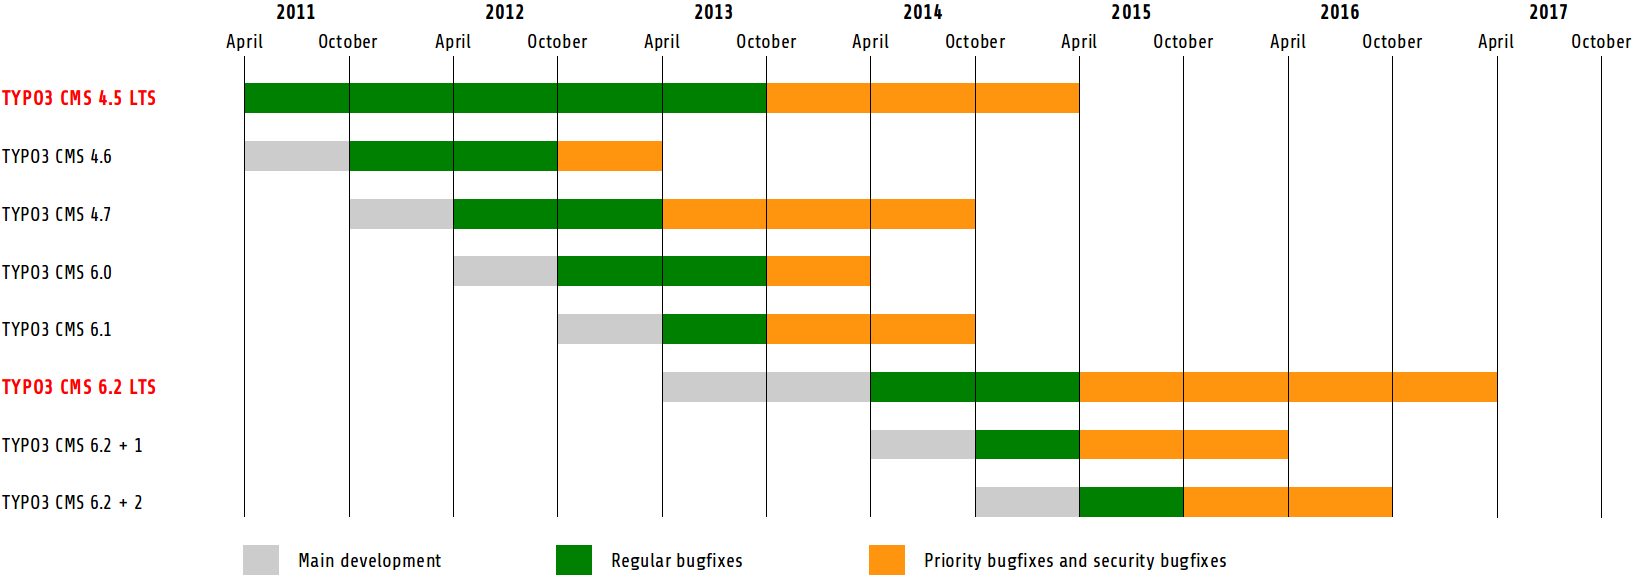
\includegraphics[width=0.90\linewidth]{Introduction/ReleaseAgenda.png}
	\end{figure}

\end{frame}

% ------------------------------------------------------------------------------
% LTXE-SLIDE-START
% LTXE-SLIDE-UID:		89710146-0b184916-c0edbb69-82032261
% LTXE-SLIDE-ORIGIN:	855168a2-d07a3cc8-65f8f9bd-827ef9e9 English
% LTXE-SLIDE-TITLE:		TYPO3 CMS Roadmap
% ------------------------------------------------------------------------------
% https://typo3.org/typo3-cms/roadmap/

\begin{frame}[fragile]
	\frametitle{Introducción}
	\framesubtitle{Línea de lanzamiento de TYPO3 CMS}

	Fechas de lanzamiento estimadas y su foco principal:

	\begin{itemize}
		\item v7.0 \textrightarrow\tabto{1.3cm}02/Dic/2014\tabto{3.4cm}Revisión Backend Vol 1

		\item
			\begingroup
				\color{typo3orange}
					v7.1 \textrightarrow\tabto{1.3cm}24/Feb/2015\tabto{3.4cm}Limpieza de Núcleo \& Coordinación
			\endgroup

		\item v7.2 \textrightarrow\tabto{1.3cm}10/Mar/2015\tabto{3.4cm}Frontend
		\item v7.3 \textrightarrow\tabto{1.3cm}21/Abr/2015\tabto{3.4cm}Ecosistema Composer
		\item v7.4 \textrightarrow\tabto{1.3cm}09/Jun/2015\tabto{3.4cm}Revisión Backend Vol 2
		\item v7.5 \textrightarrow\tabto{1.3cm}28/Jul/2015\tabto{3.4cm}\textit{(por determinar...)}
		\item v7.6 \textrightarrow\tabto{1.3cm}13/Oct/2015\tabto{3.4cm}pre-LTS inferno
		\item v7.7 \textrightarrow\tabto{1.3cm}xx/xxx/2015\tabto{3.4cm}\textbf{TYPO3 CMS 7 LTS} (Soporte a Largo Plazo)
	\end{itemize}

	\smaller
		\url{https://typo3.org/typo3-cms/roadmap/}\newline
		\url{http://typo3.org/news/article/embrace-and-innovate-typo3-cms-7/}
	\normalsize

\end{frame}

% ------------------------------------------------------------------------------
% LTXE-SLIDE-START
% LTXE-SLIDE-UID:		f9d62780-efd4f19d-34c4115f-47d68f7e
% LTXE-SLIDE-ORIGIN:	0a54fbe0-06a2837d-605a5eed-6aa40506 English
% LTXE-SLIDE-TITLE:		Installation
% LTXE-SLIDE-REFERENCE:	https://forge.typo3.org/issues/62578
% ------------------------------------------------------------------------------

\begin{frame}[fragile]
	\frametitle{Introducción}
	\framesubtitle{Instalación}

	\begin{itemize}
		\item Procedimiento de instalación oficial bajo Linux/Mac OS X\newline
			(DocumentRoot por ejemplo \texttt{/var/www/site/htdocs}):
		\begin{lstlisting}
			$ cd /var/www/site
			$ wget --content-disposition get.typo3.org/7.1
			$ tar xzf typo3_src-7.1.0.tar.gz
			$ cd htdocs
			$ ln -s ../typo3_src-7.1.0 typo3_src
			$ ln -s typo3_src/index.php
			$ ln -s typo3_src/typo3
			$ touch FIRST_INSTALL
		\end{lstlisting}

		\item Enlaces simbólicos bajo Microsoft Windows:

			\begin{itemize}
				\item Use \texttt{junction} bajo Windows XP/2000
				\item Use \texttt{mlink} bajo Windows Vista and Windows 7
			\end{itemize}

	\end{itemize}
\end{frame}

% ------------------------------------------------------------------------------
% LTXE-SLIDE-START
% LTXE-SLIDE-UID:		0981410f-2b0b234e-0a3b7ec8-90f49a37
% LTXE-SLIDE-ORIGIN:	914dda49-a07eaf35-b9d24c58-6890a673 English
% LTXE-SLIDE-TITLE:		Upgrade to TYPO3 CMS 7
% LTXE-SLIDE-REFERENCE:	https://forge.typo3.org/issues/62578
% ------------------------------------------------------------------------------

\begin{frame}[fragile]
	\frametitle{Introducción}
	\framesubtitle{Actualización a TYPO3 CMS 7.x}

	\begin{itemize}
		\item Actualizaciones sólo posibles desde TYPO3 CMS 6.2 LTS
		\item TYPO3 CMS < 6.2 debe ser actualizado a TYPO3 CMS 6.2 LTS primero
	\end{itemize}

	\begin{itemize}

		\item Instrucciones de Actualización:\newline
			\smaller\url{http://wiki.typo3.org/Upgrade#Upgrading_to_7.1}\normalsize
		\item Guía oficial de TYPO3 "Instalación y Actualización de TYPO3":
			\smaller\url{http://docs.typo3.org/typo3cms/InstallationGuide}\normalsize
		\item Enfoque general:
			\begin{itemize}
				\item Comprobar requisitos mínimos del sistema \small(PHP, MySQL, etc.)
				\item Revisar \textbf{deprecation\_*.log} en vieja instancia de TYPO3
				\item Actualizar todas las extensiones a la última versión
				\item Desplegar nuevas fuentes y correr la Herramienta de Instalación \textrightarrow Asistente de Actualización
				\item Revisar módulo de inicio para usuarios del backend (opcionalmente)
			\end{itemize}
	\end{itemize}

\end{frame}

% ------------------------------------------------------------------------------
